%!Tex Program = xelatex
\documentclass[a4paper]{article}
%\documentclass[a4paper]{ctexart}
\usepackage{xltxtra}
%\setmainfont[Mapping=tex-text]{AR PL UMing CN:style=Light}
%\setmainfont[Mapping=tex-text]{AR PL UKai CN:style=Book}
%\setmainfont[Mapping=tex-text]{WenQuanYi Zen Hei:style=Regular}
%\setmainfont[Mapping=tex-text]{WenQuanYi Zen Hei Sharp:style=Regular}
%\setmainfont[Mapping=tex-text]{AR PL KaitiM GB:style=Regular} 
%\setmainfont[Mapping=tex-text]{AR PL SungtiL GB:style=Regular} 
\usepackage{graphicx}
\usepackage{fontspec}
\usepackage{cite}
\usepackage{geometry}

% 设置中文字体
\setmainfont{AR PL UMing CN}

\geometry{left=20mm,right=20mm,top=20mm,bottom=20mm}

\begin{document}


\title{最小二乘拟合示例}
\author{水煮鱼}
\date{\today}
\maketitle

\section{介绍}

最小二乘拟合是一种数学方法, 用于寻找最佳拟合曲线或直线, 使得观测数据点
与预测值之间的平方差之和最小化~\cite{ref1,ref2}. 它常用于估计线性回归
模型的参数.

在本示例中, 我们展示了最小二乘拟合方法在一组数据点上的应用. 我们计算了
最佳拟合直线的斜率和截距, 并将其与数据点一起绘制.

\section{数据和拟合结果}

图 \ref{fig:fitting} 显示了从分析中获得的数据点和最小二乘拟合直线.

\begin{figure}[htbp]
    \centering
    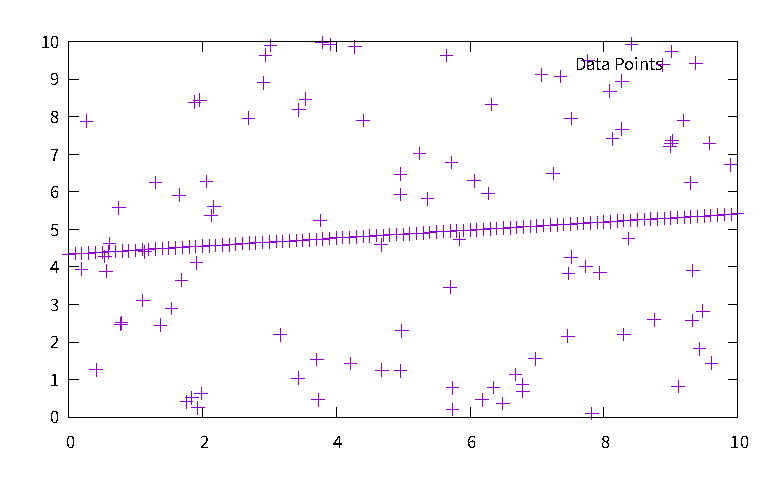
\includegraphics[width=0.8\textwidth]{output.eps}
    \caption{最小二乘拟合}
    \label{fig:fitting}
\end{figure}

最佳拟合直线的斜率和截距计算如下:

\noindent 斜率: 2.15

\noindent 截距: 0.62

\section{结论}

最小二乘拟合方法提供了一种寻找最佳拟合直线的方式, 使得观测数据点与预测
值之间的平方差之和最小化~\cite{ref1}. 它在统计学、工程学和数据分析等领
域中具有广泛的应用.

% 使用 BibTeX 管理文献引用
\bibliographystyle{plain}
\bibliography{references}

\end{document}

